%csky stuff
\chapter{Time-Integrated Search}

\section{Analysis properties}


\subsection{Background space PDF}

\begin{figure}
    \centering
    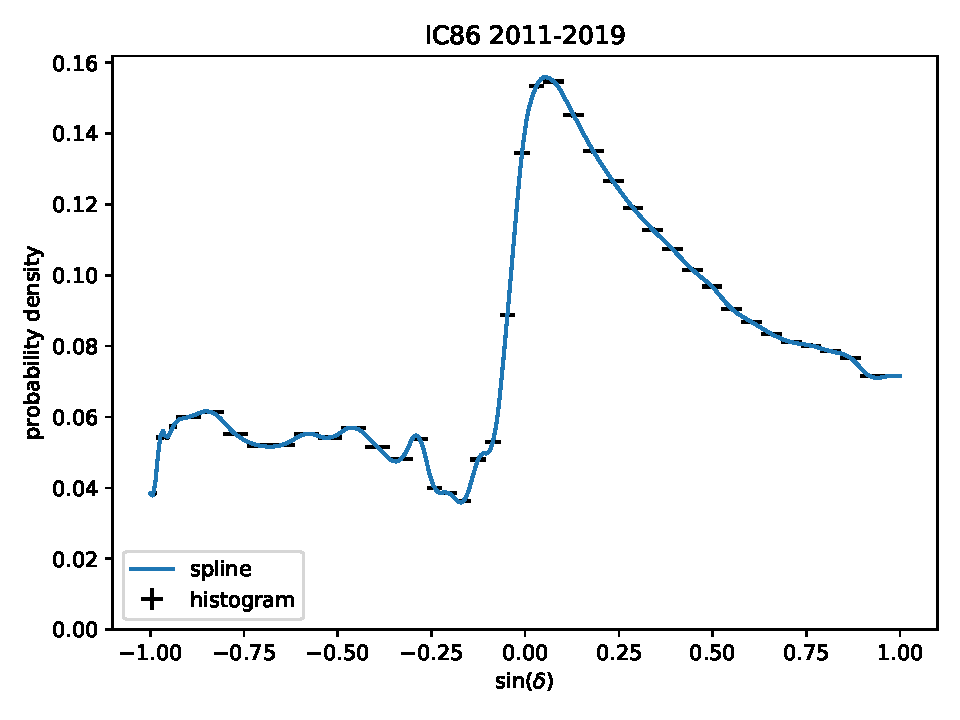
\includegraphics[width=\linewidth]{Plots/05_csky/bg_space_pdf.pdf}
    \caption{Background space PDF used in this analysis in $\sin{(\delta)}$ for all $\num{9}$ years, 2011-2019.}
\end{figure}

The background space parametrization results in one plot only because all datasets underwent the same data processing pipeline.

\subsection{Energy ratio PDF}

\begin{figure}
    \centering
    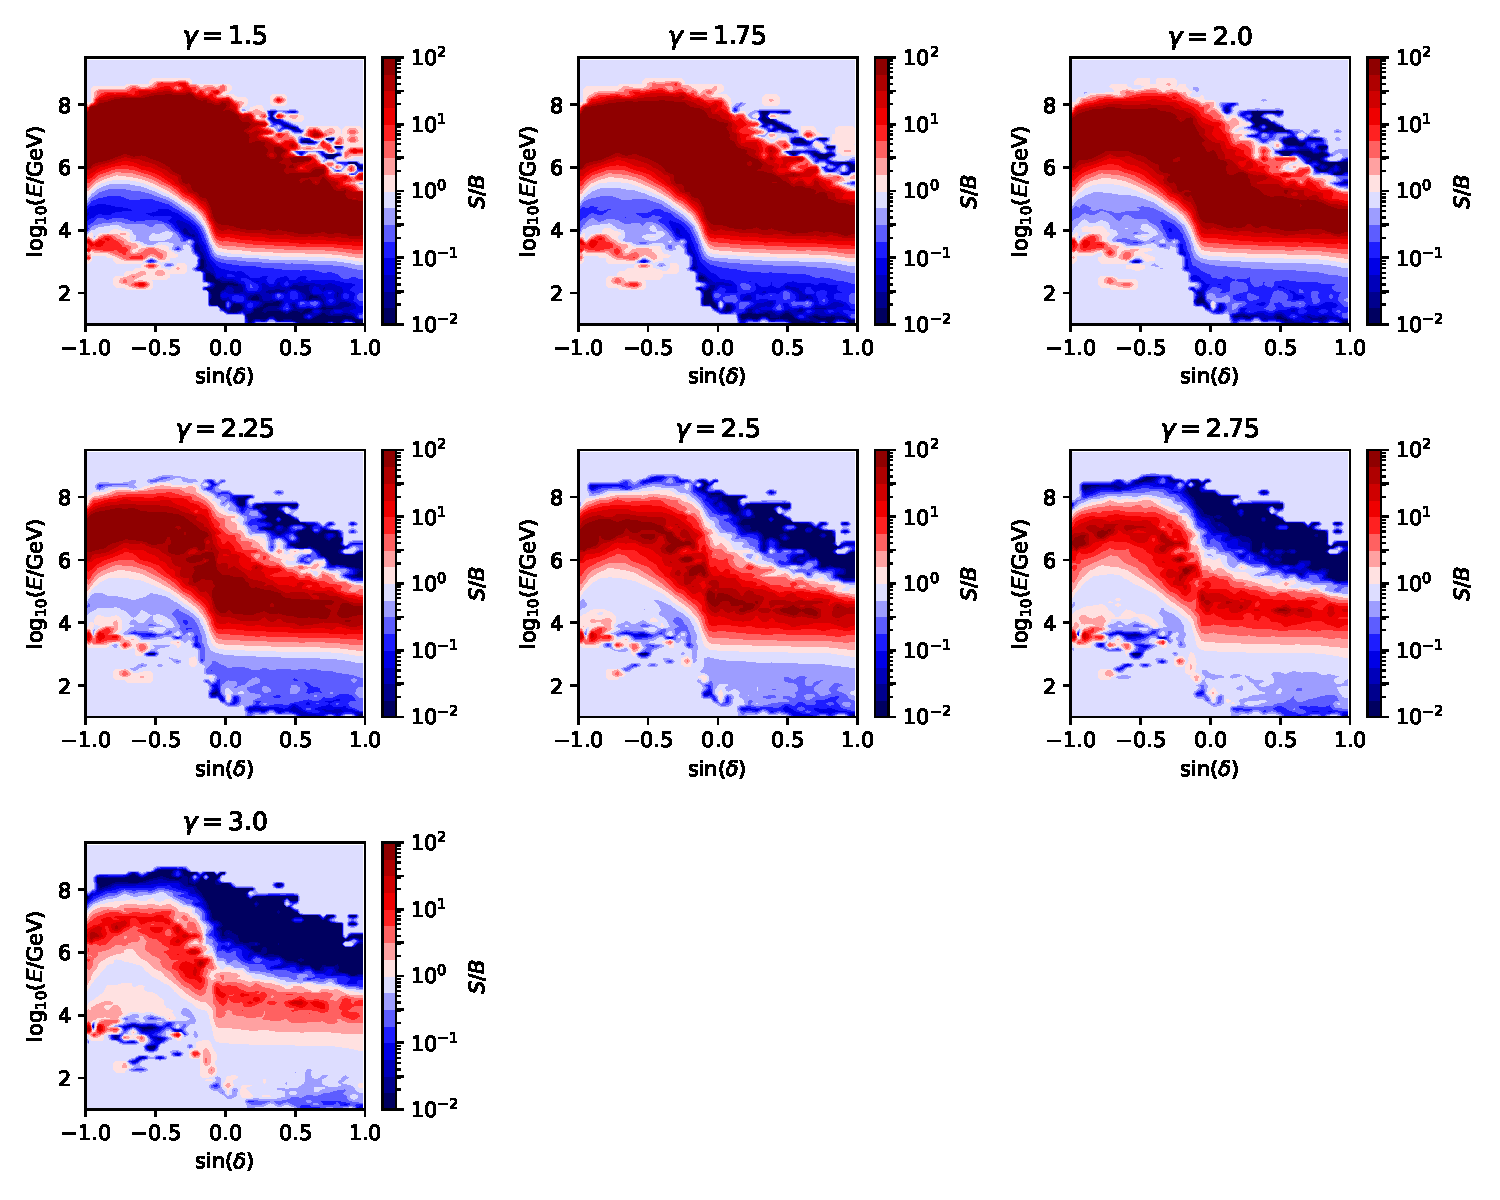
\includegraphics[width=\linewidth]{Plots/05_csky/energy_pdf_ratio.pdf}
    \caption{Energy PDF ratios used in this analysis in $\sin{(\delta)}$ and $\sin{\log{(E)}}$ for all $\num{9}$ years, 2011-2019, for different spectral indices $gamma$.}
\end{figure}

\section{Background Trials}

The histogram of the background test statistic values can be seen in figure \ref{fig:bg_ts_time_int}.
The number of trials processed is $\num{974000}$\footnote{Originally $\num{e6}$, but some jobs fail due to various technical reasons.}.
Important features of the plot are that the $\chi^2$ distribution has as straight a tail as possible.
This is reflected in the number of degrees of freedom $dof$ in the $\chi^2$ distribution.
This should be as close to 1 as possible, which corresponds to a pure background statistic without signal.
The test statistic should also be symmetrical around the zero point.
A shift around the zero point is an indication of an undesired bias of the statistic.
Therefore, the value of the quotient of the number of positive and negative events should ideally be $\eta = \num{0.5}$.
Apart from the fit parameters, the median and $5\sigma$ deviation value of the test statistic are necessary for the subsequent calculation of the sensitivity and the discovery potential.

The fit parameters of the background test statistic are
\begin{align}
  dof &= \num{1.115},\\
  \eta &= \num{0.656}
\end{align}
and the key values later to be processed are as follows\footnote{Some analyses use the $3\sigma$ value for the discovery potential}
\begin{align}
  median &= \num{0.140},\\
  3\sigma &= \num{10.651},\\
  5\sigma &= \num{28.060}.
\end{align}

\begin{figure}
    \centering
    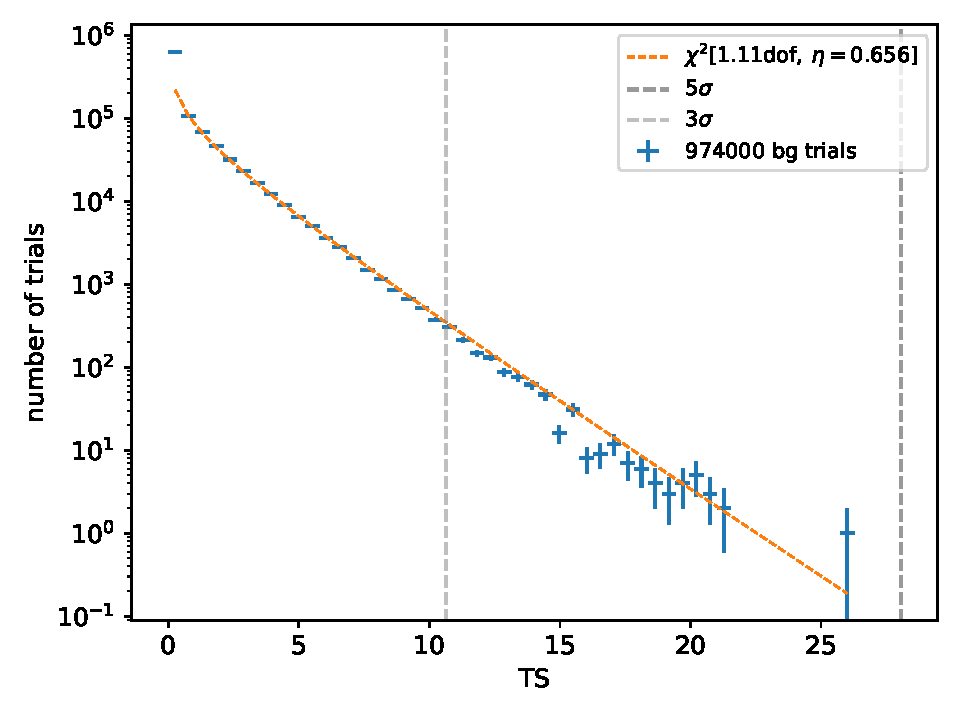
\includegraphics[width=\linewidth]{Plots/05_csky/9_years_gfu_gold_bg_new.pdf}
    \caption{Histogram of the background test statistic for the time integrated analysis. Shown are also the number of degrees of freedom $dof$ and the ratio of positive and negative values $\eta$.}
    \label{fig:bg_ts_time_int}
\end{figure}

\section{Signal Trials}

\begin{figure}
    \centering
    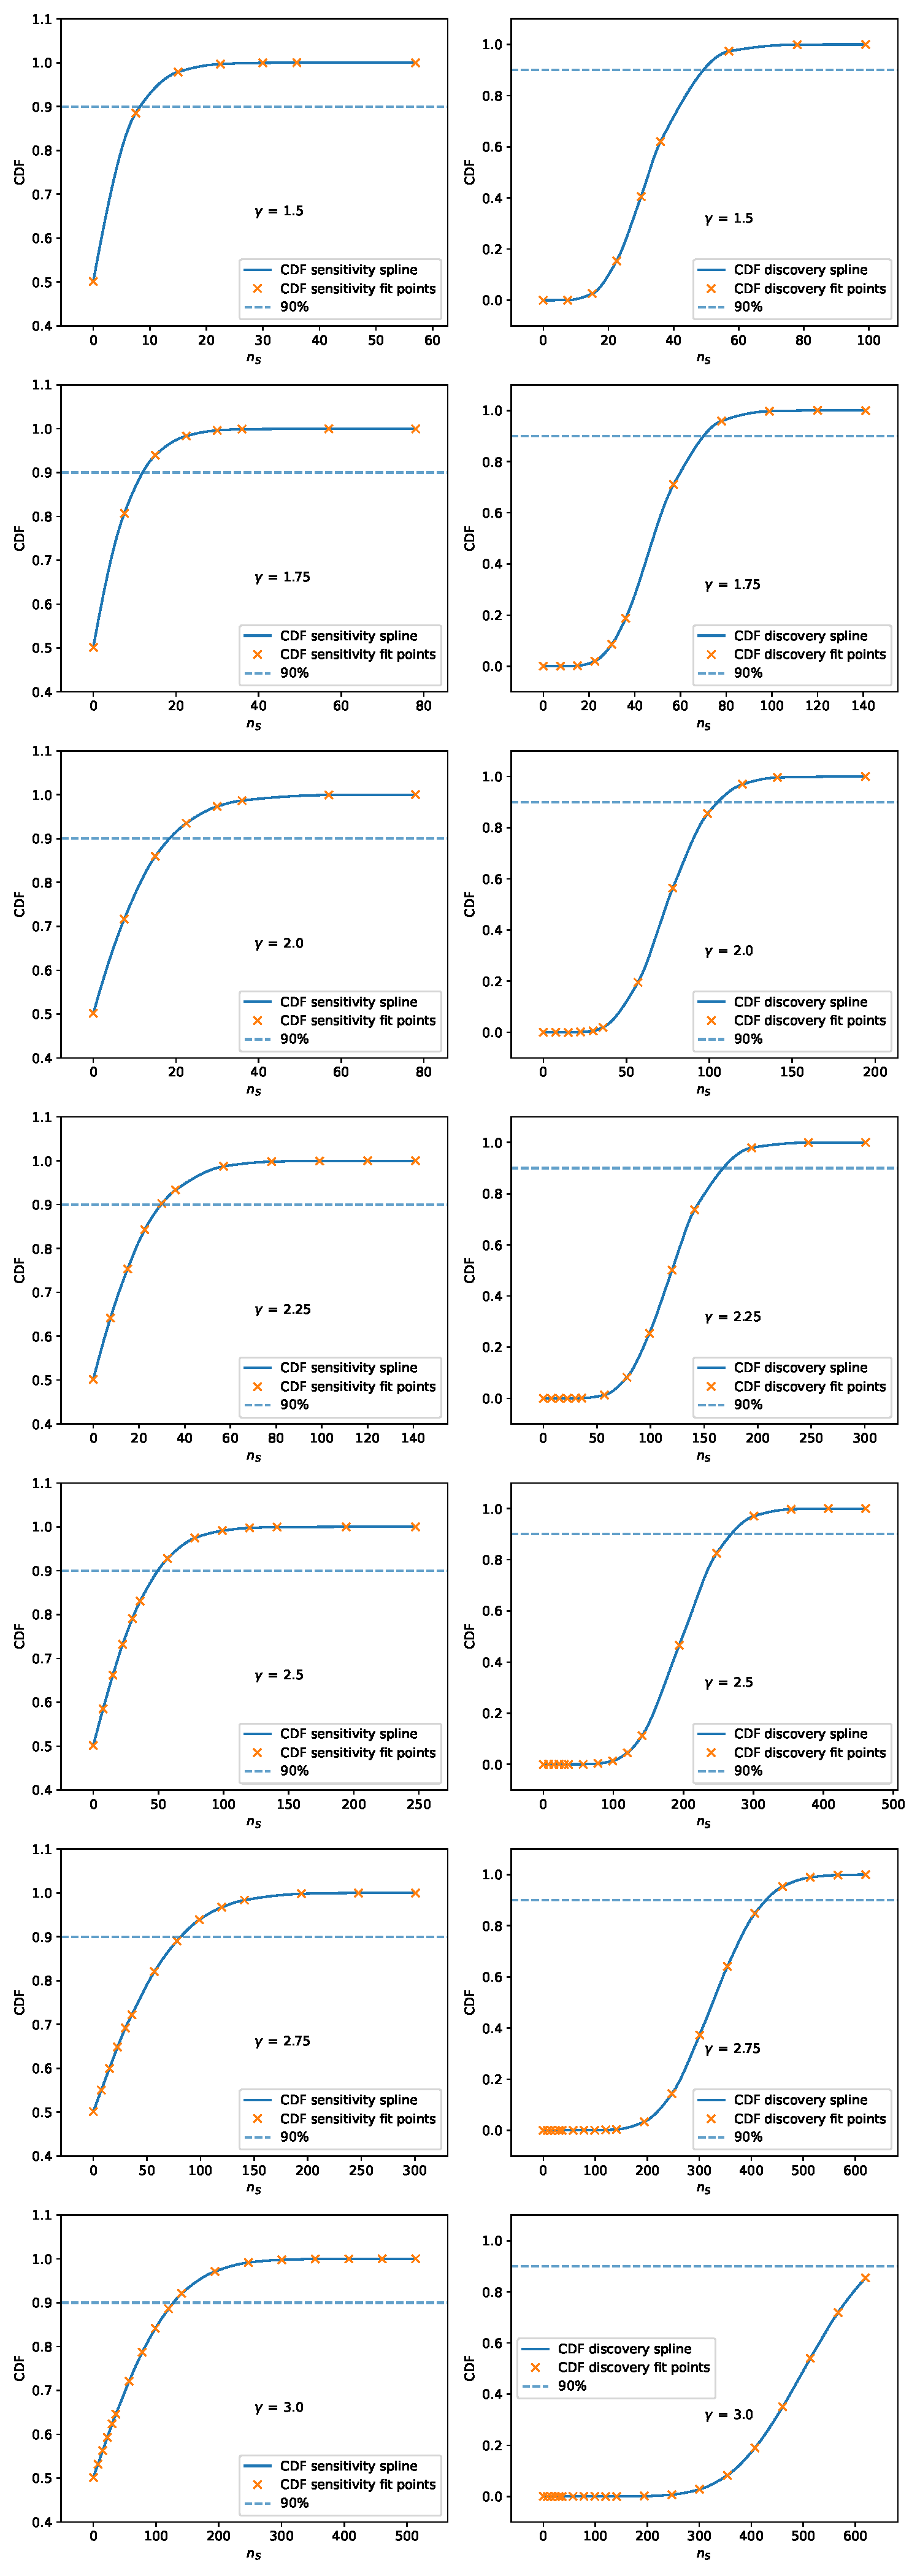
\includegraphics[width=5cm]{Plots/05_csky/9_years_gfu_gold_cdf.pdf}
    \caption{.}
\end{figure}

\begin{figure}
    \centering
    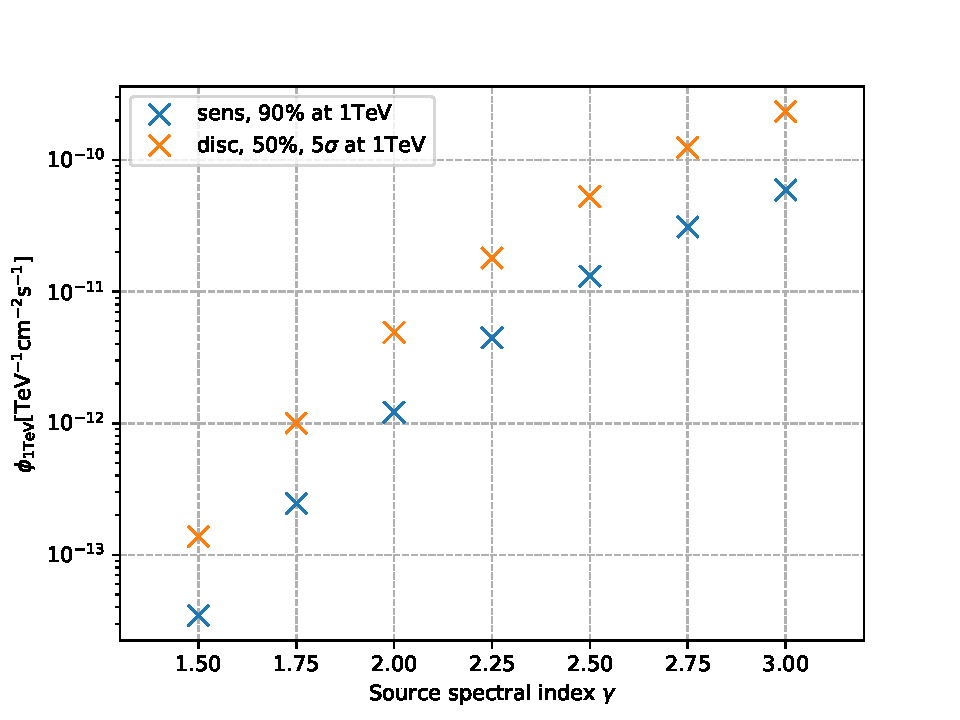
\includegraphics[width=5cm]{Plots/05_csky/time_int_sens_gfu_gold_9_years_new.pdf}
    \caption{.}
\end{figure}

\chapter{Time-Dependent Search}

\section{Background Trials}

\begin{figure}
    \centering
    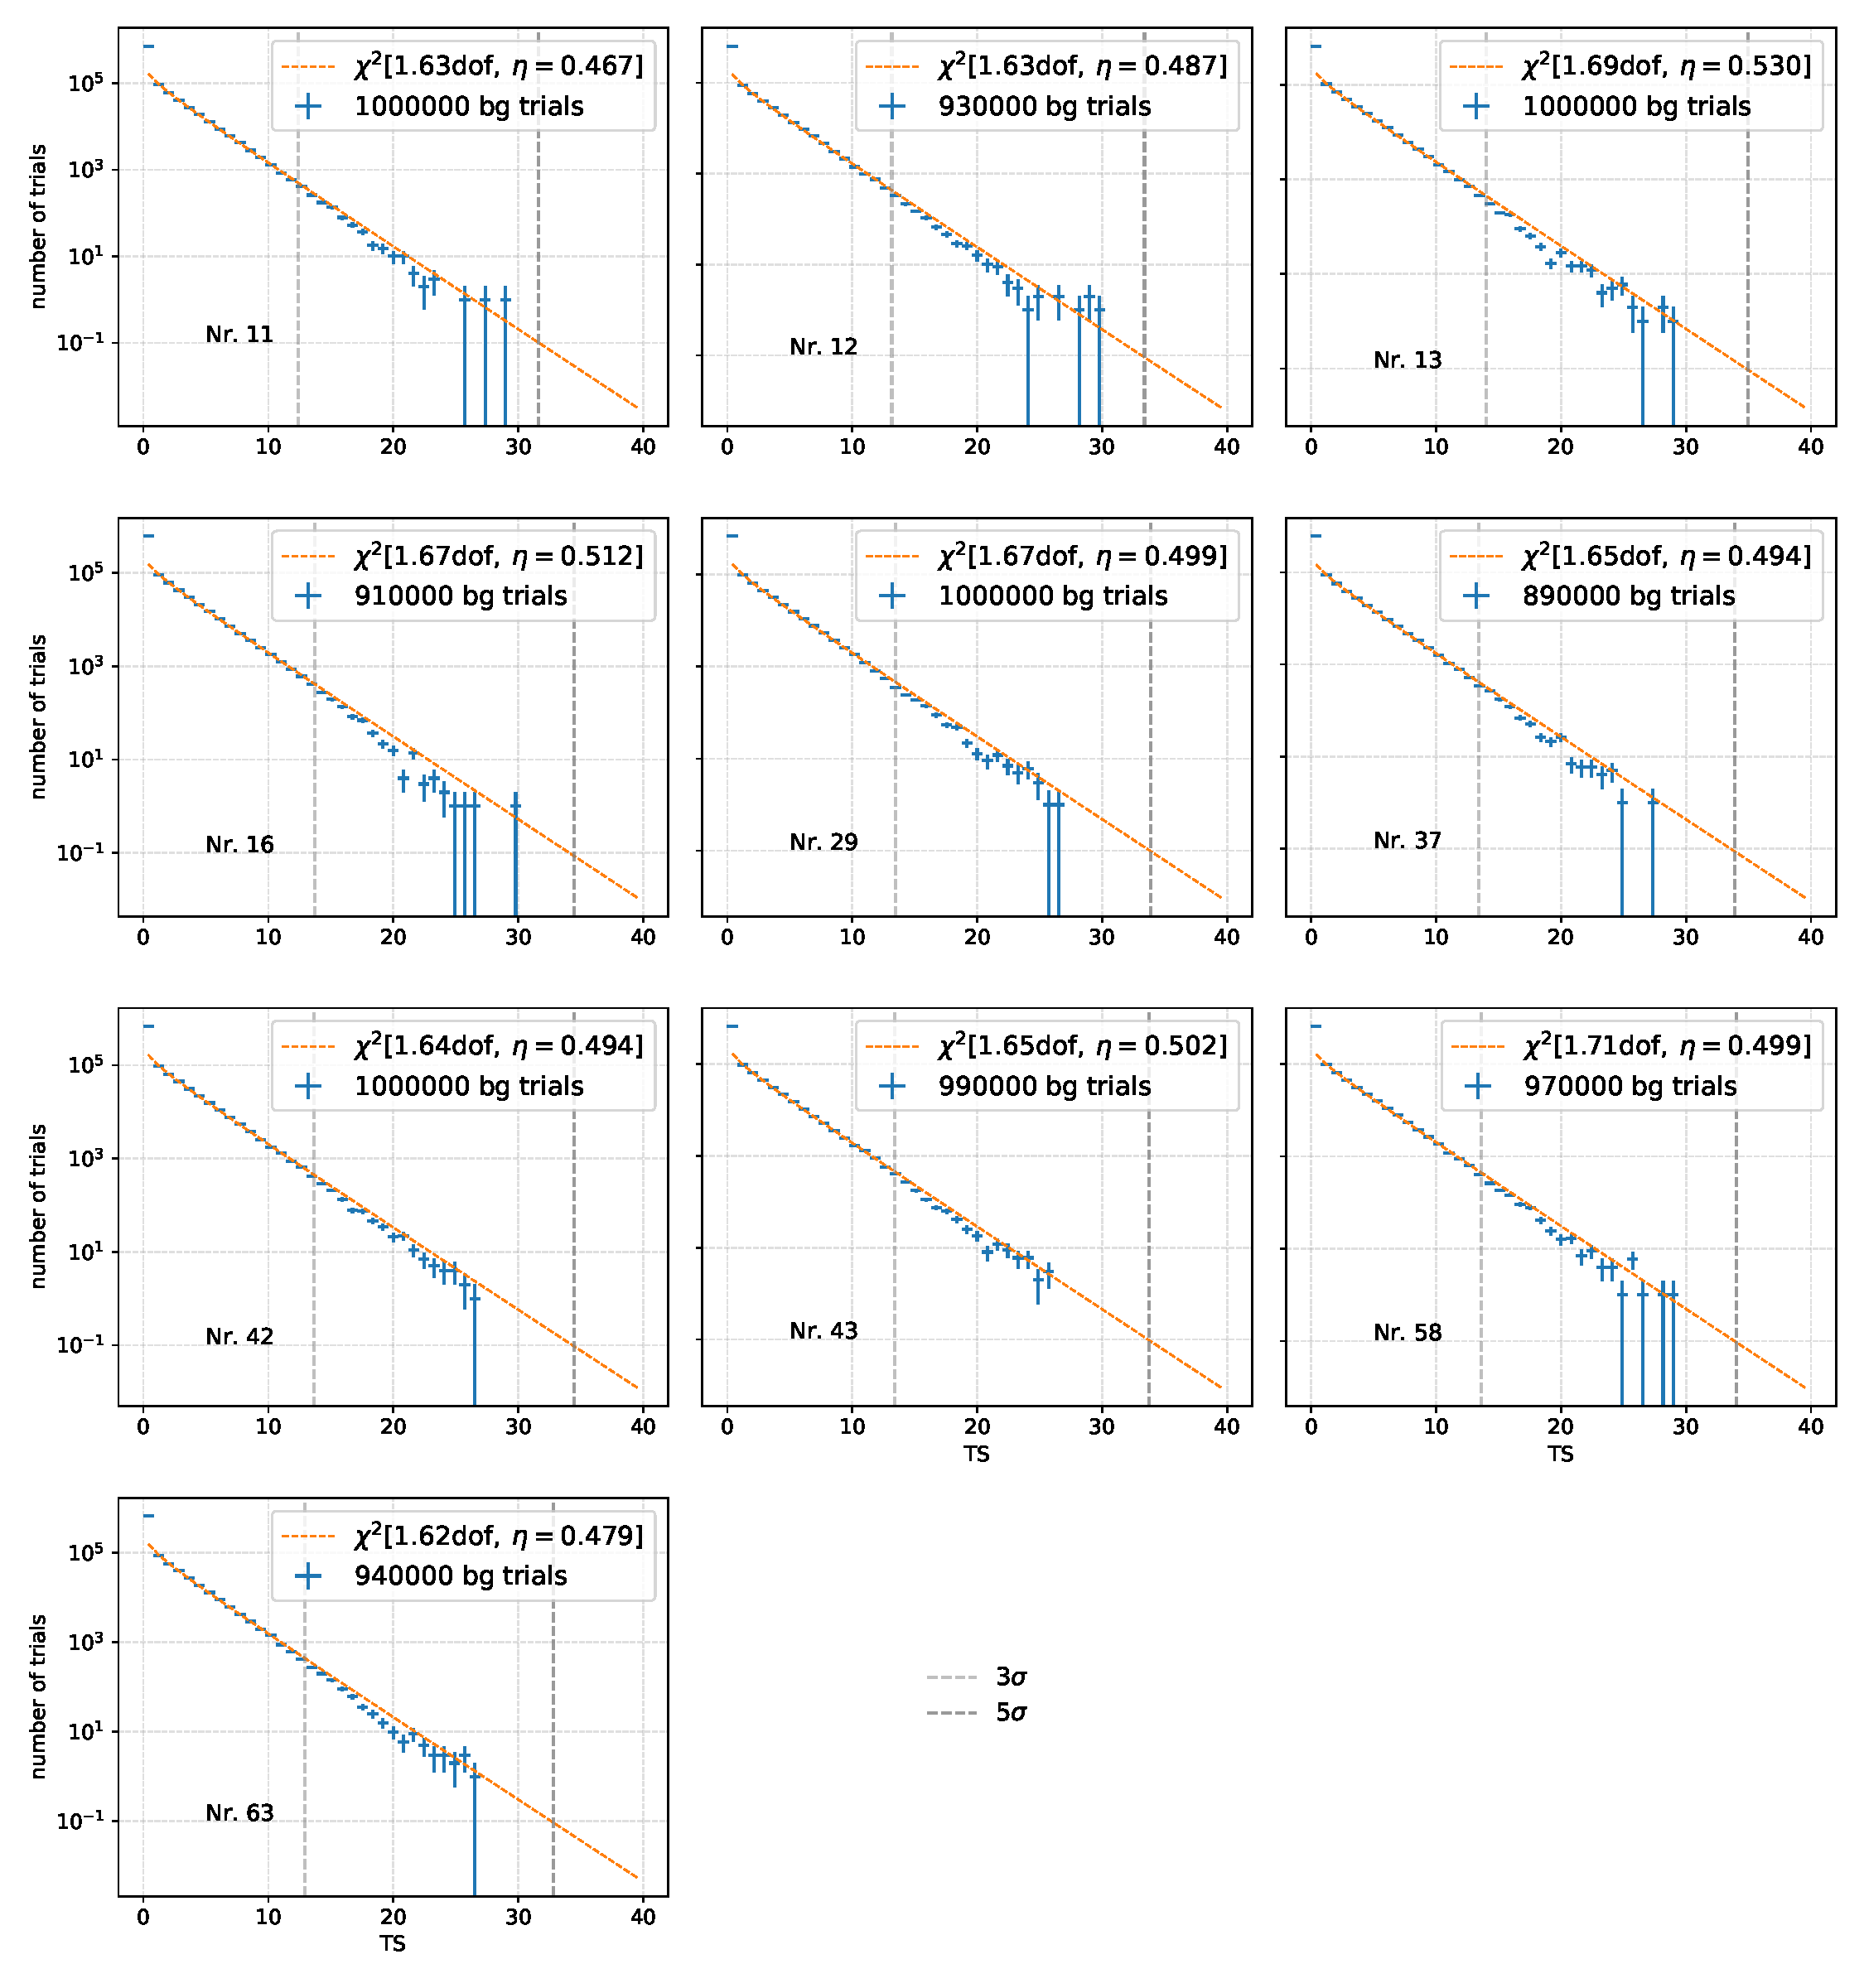
\includegraphics[width=5cm]{Plots/05_csky/9_years_gfu_gold_time_dep_bg_t0.pdf}
    \caption{.}
\end{figure}

\begin{figure}
    \centering
    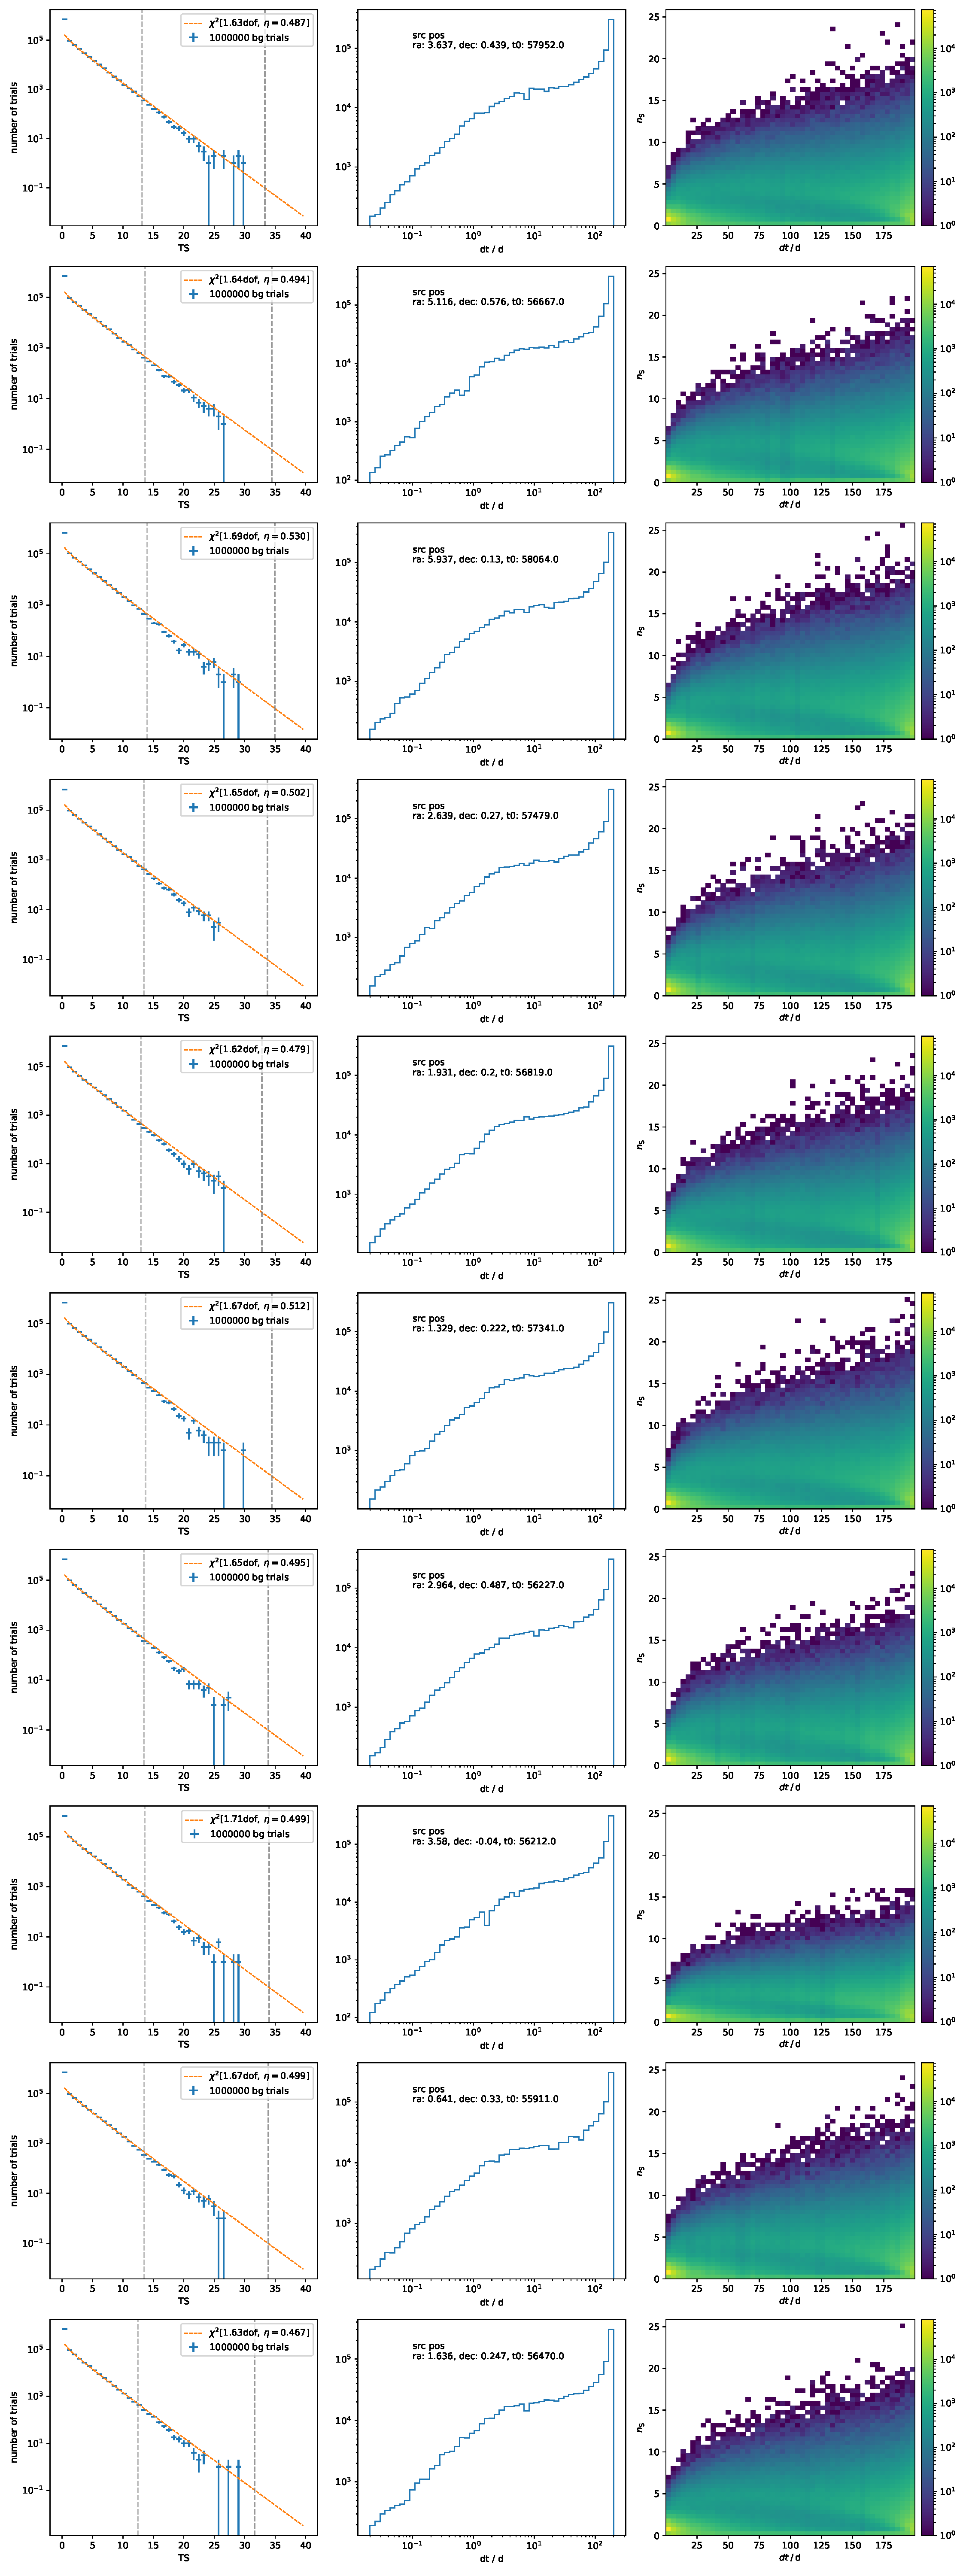
\includegraphics[width=5cm]{Plots/05_csky/9_years_gfu_gold_time_dep_bg_timewindows_fixed_t0.pdf}
    \caption{.}
\end{figure}

ns = 2 because the time box is set between 2 events, thus ns = 2 and maybe lower because of weighting (events may not look as signal like)
\section{Signal Trials}

\begin{figure}
    \centering
    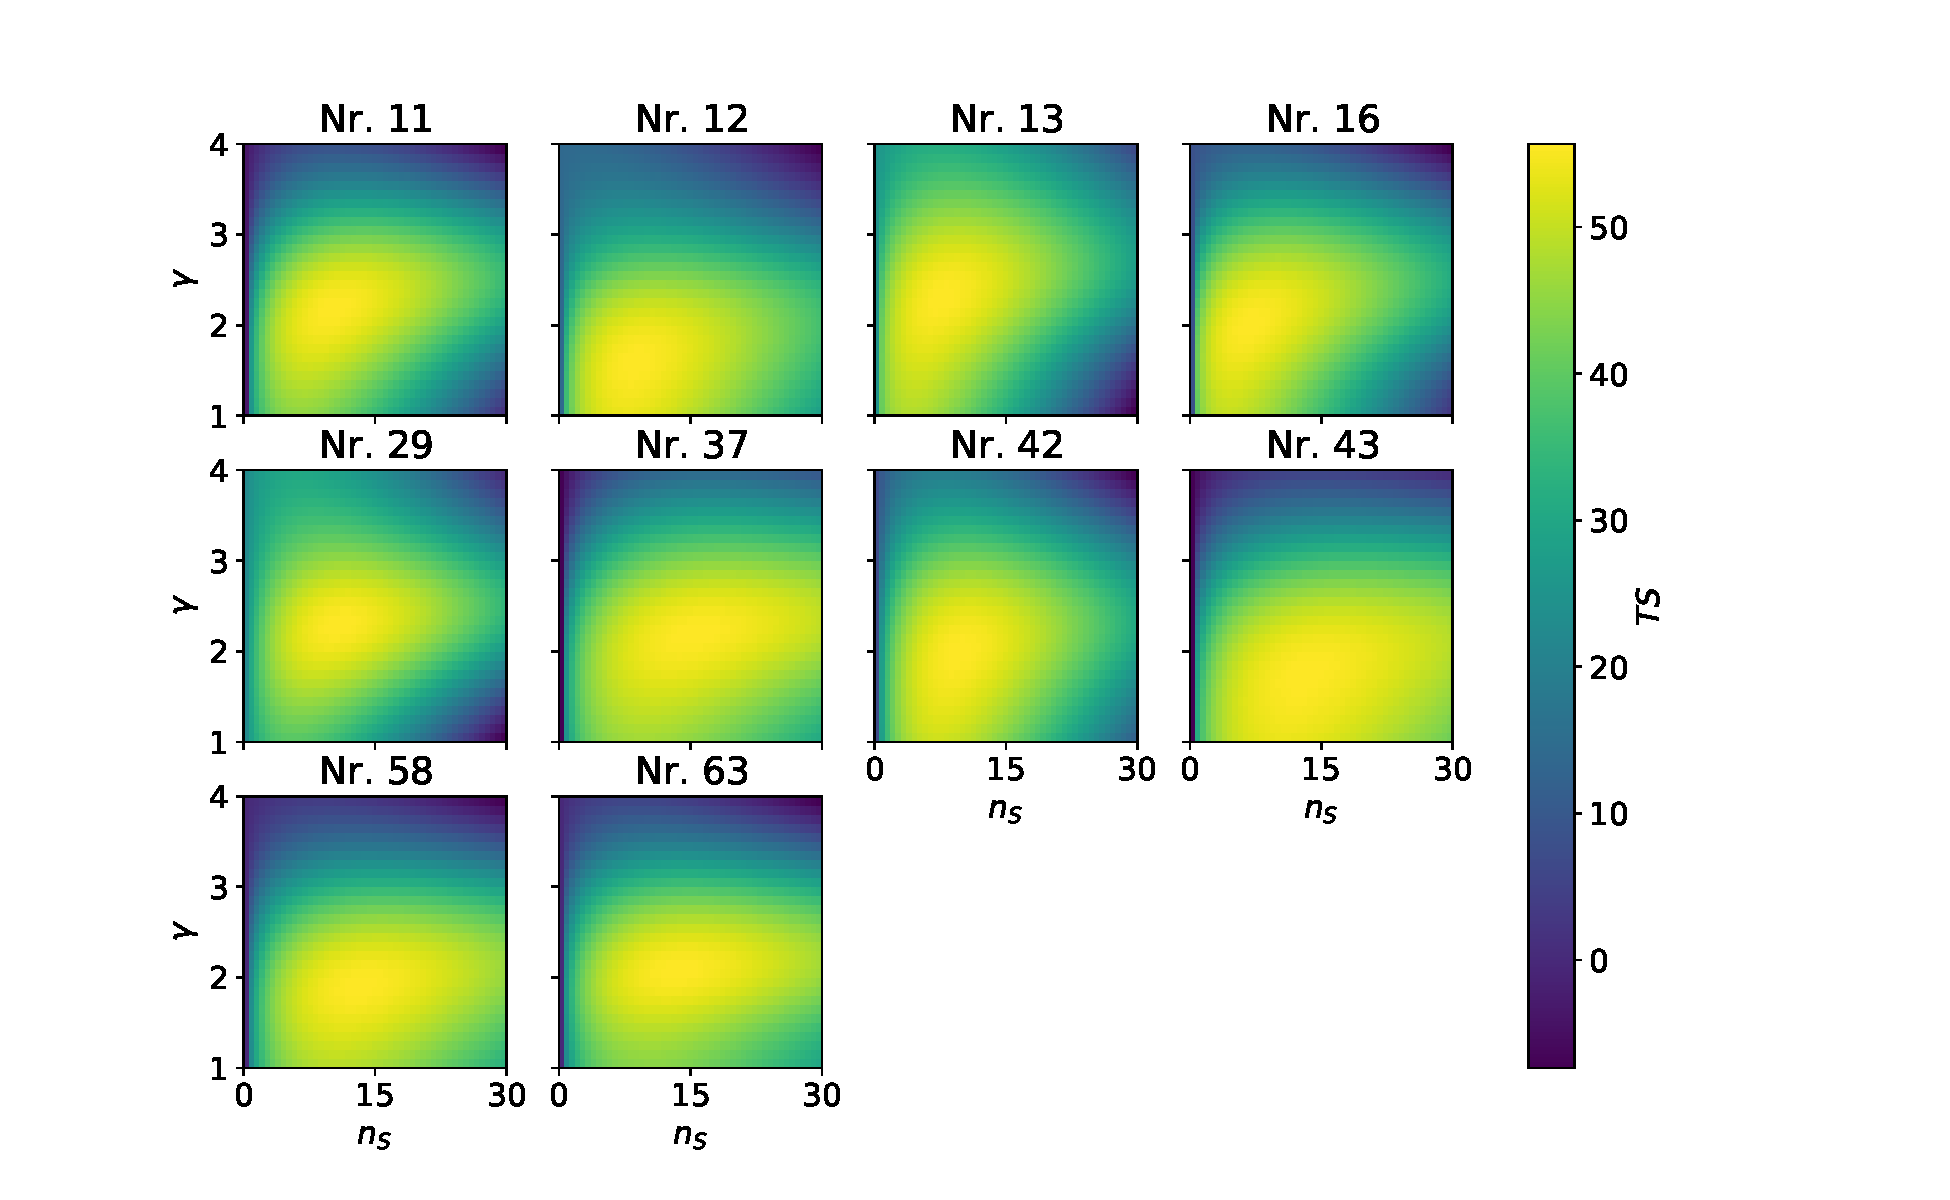
\includegraphics[width=\linewidth]{Plots/05_csky/llh_scan.pdf}
    \caption{Scan of the likelihoodspace for every source with a timewindow of $\SI{200}{\day}$. The scan is in the spectral index $\gamma$ and the signal parameter $n_S$. The source number corresponds to table \ref{tab:sources}.}
\end{figure}
